In today's problems, 
we're going to investigate how to use \myEmph{higher degree} polynomials 
to fit some $(x,y)$ data ``really, really well''.

\section*{One Dataset, Five Regression Models}

\begin{minipage}{0.5\textwidth}
    Here are the data you will use to answer all the questions.
\end{minipage}
\begin{minipage}{0.29\textwidth}
\begin{center}
    \Large
    \begin{tabular}{cc}
        \toprule 
        $x$ & $y$ \\ 
        \midrule
        0.00 & -3.00 \\
        2.00 & 14.96 \\
        4.00 & 19.94 \\
        6.00 & 10.12 \\
        8.00 & 55.06 \\
        10.00 & 64.70 \\
        \bottomrule
    \end{tabular}
\end{center}
\end{minipage}

Here are the polynmial models\footnote{
    Notice that there are \myEmph{subscripts} on the parameters
    ($a_1, b_1, c_1, \dots, a_2, b_2, c_2\dots$).
    That way, the parameters are different for each model, 
    and you can put them all into \myDesmos once and reuse them for each problem.
}
we will use.
\begin{center}
\footnotesize
\renewcommand{\arraystretch}{2}
\begin{tabular}{r||l|l}
    \toprule
    {model} 
        & {\myDesmos command} 
        & {model} \\
    \midrule 
    {\itshape Linear} 
        & {\ttfamily
            y1 $\sim$ a1 + b1 x1
        }
        & $y = \bm{a_1} + \bm{b_1}x$
        \\
    {\itshape Quadratic} 
        & {\ttfamily
            y1 $\sim$ a2 + b2 x1 + c2 x1\textasciicircum 2
        }
        & $y = \bm{a_2} + \bm{b_2}x + \bm{c_2}x^2$
        \\
    {\itshape Cubic} 
        & {\ttfamily
            y1 $\sim$ a3 + b3 x1 + c3 x1\textasciicircum 2 + d3  x1\textasciicircum 3
        }
        & $y = \bm{a_3} + \bm{b_3}x + \bm{c_3}x^2 + \bm{d_3}x^3$
        \\
    {\itshape Quartic} 
        & {\ttfamily
            y1 $\sim$ a4 + b4 x1 + c4 x1\textasciicircum 2 + d4  x1\textasciicircum 3 + \fbox{f4}  x1\textasciicircum 4
        }
        & $y = \bm{a_4} + \bm{b_4}x + \bm{c_4}x^2 + \bm{d_4}x^3 + \boxed{\bm{f_4}}x^4$
        \\
    {\itshape Quintic} 
        & {\ttfamily
        y1 $\sim$ a5 + b5 x1 + c5 x1\textasciicircum 2 + d5  x1\textasciicircum 3 + \fbox{f5}  x1\textasciicircum 4 + \fbox{g5}  x1\textasciicircum 5
        }
        & $y = \bm{a_5} + \bm{b_5}x + \bm{c_5}x^2 + \bm{d_5}x^3 + \boxed{\bm{f_5}}x^4 + \boxed{\bm{g_5}}x^5$
        \\
    \bottomrule
\end{tabular}
\end{center}

\begin{tcolorbox}[center,width=5in,]
    \myEmph{Do not} use $\bm{e_i}$ as one of your parameters.\\[0.5\onelineskip]
    \myDesmos treats this as something called {\itshape residuals}
    (literally ``stuff left over'').
    We \myEmph{won't} talk about residuals, but they are covered in the {\itshape Statistics} class.
\end{tcolorbox}


\myProblemsWithContent
{
    Sketch a scatterplot of the $(x,y)$ data.\newline
        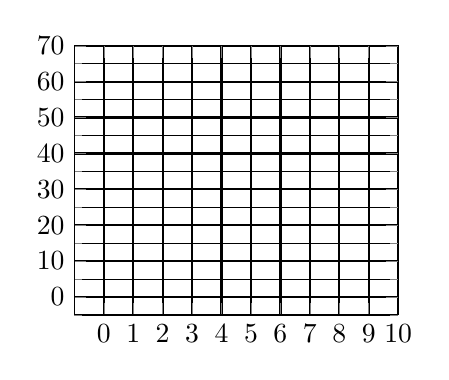
\begin{tikzpicture}
            \begin{axis}[
                scale=0.6,
                grid = both,
                xmin=-1, xmax=10, xtick distance=1, xtickmin=0,
                ymin=-5, ymax=70, ytick distance=10, minor y tick num=1,
                major grid style={solid,thick,black},
                minor grid style={solid,very thin,black},
            ]
            \end{axis}
        \end{tikzpicture}
    % \end{center}
    % \end{minipage}  
}
{
    Do these points seem to be linear or something else? Explain your thinking.
}[\small]